\chapter{Compilation and Linking}
The process that bridges the source code to machine code and the final executable is the compilation; human readable
code is translated into binary instructions that can be read and executed by the CPU. The compilation of C code for
instance requires 4 steps:
\begin{enumerate}
    \item Preprocessing;
    \item Compilation;
    \item Assembly;
    \item Linking.
\end{enumerate}
Most of the times these phases are merged into a single one by modern compilers but in reality they are carried out
separately.
\begin{figure}[!htbp]
    \centering
    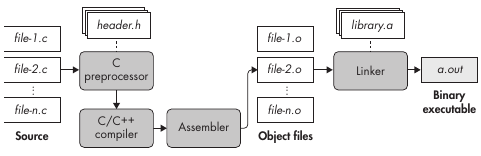
\includegraphics[scale=0.7]{./pics/compilation.png}
    \caption{Compilation phases}
    \label{comp}
\end{figure}

\subsection{Preprocessing}
The source files to be compiled normally contains a certain number of macros (denoted by the {\ttfamily \#define})
keyword and {\ttfamily \#include} directives; in the preprocessing phase these are expanded (i.e. macros and header
files are translated into equivalent C source code). At this stage all of the headers have been "copied" into our
source code ands ready to be compiled. In gcc the output of the preprocessing step can be obtained by issuing the
command {\ttfamily gcc -E -P}.

\subsection{Compilation}
The compilation phase translates the processed source code into assembly language. At this stage it is possible to
invoke compiler optimisation on our code (for gcc, clang and most of the UNIX toolchain the optimisation options
range in {\ttfamily -O0-3}). Compiling directly into machine code would be too much of a daunting, if not plain
risky, task; thus it is better to have a single dedicated assembler that can handle the final translation into
machine code. The output of the compilation phase is indeed pretty much human readable with intact symbolic
information. In order to tell the compiler to stop at this stage we can issue the {\ttfamily -S masm=intel} options to
obtain the assembly file (*.s).
